
%$$$$$$$$$$$$$$$$$$$$$$$$$$$$$$$$$$$$$$$$$$$$$$$$$$$$$$$$$$$$$$$$$$$$$$$$$$$$$$$$
%Paragraph 2:Concurrent updates에 대한 연구
%$$$$$$$$$$$$$$$$$$$$$$$$$$$$$$$$$$$$$$$$$$$$$$$$$$$$$$$$$$$$$$$$$$$$$$$$$$$$$$$$
\newpage
\section{확장성 있는 자료구조 연구}
\label{sec:datarelated}
%Many scalable data structures with scalable schemes show different performances
% depending on their update ratios.
많은 확장성 있는 방법과 사용되는 자료구조들은 업데이트 비율에 따라 다른 성능을 가진다.  
%In low and middle update rate, researchers have attempted to create new
% scalable schemes~\cite{McKenney98}~\cite{Matveev2015RLU}~\cite{Harris2001Lockfree}
%~\cite{Fomitchev2004Lockfree}
%~\cite{Timnat2012}
%or have attempted to adapt these scheme to data
%structures~\cite{Arbel2014ConcurrentRCU}~\cite{Dodds2015SCT}~\cite{AustinTClements2012RCUBalancedTrees}.
낮거나 중간 정도의 업데이트 비율에서는 연구자들은 새로운 확장성있는
기법~\cite{McKenney98}~\cite{Matveev2015RLU}~\cite{Harris2001Lockfree} ~\cite{Fomitchev2004Lockfree}
~\cite{Timnat2012}을 연구하거나 그 기법을 자료구조에 
적용~\cite{Arbel2014ConcurrentRCU}~\cite{Dodds2015SCT}~\cite{AustinTClements2012RCUBalancedTrees}을
하도록 시도하고 있다.
%In high update rate, the OpLog shows significant improvement in
%performance scalability for update-heavy data structures in
%many core systems, but suffers from limitation and overhead due
%to time-stamp counter management.
높은 업데이트 비율에서는 OpLog가 매니코어의 업데이트 비율이 높은 자료 구조에 대해서
 상당히 높은 성능 확장성을 가진다. 
%We substantially extend our preliminary work~\cite{Kyong2016LDU} not only to
% support per-core algorithm but also to apply the \LDU to anonymous rmap due to improving the
%Linux kernel scalability.

\subsection{확장성 있는 자료구조를 위한 동기화 기법}

\subsubsection{RCU}


확장성을 위한 대표적 동기화 기법인 RCU는 McKenney와 Slingwine에 의해 개발되었고,
 동기화 기법 때문에 발생하는 오버헤드를
최소화 시킨 방법이다.
특히 RCU는 리더들을 보호하기 위해 사용하는 동기화 기법의 오버헤드를 최소화 시킨다.
단점으로는 RCU의 라이터가 가 수행하는 방법은 복잡하고 느리다. 
이러한 단점에도 불구하고 리더들이 수행하는 락의 오버헤드가 적고, 여러 리더와 
업데이터 하나가 동시에 수행이 가능하므로 RCU는 현재 리눅스 커널에서 상당히 많이 사용되고 있다. 


\begin{figure}[h]
    \centering
    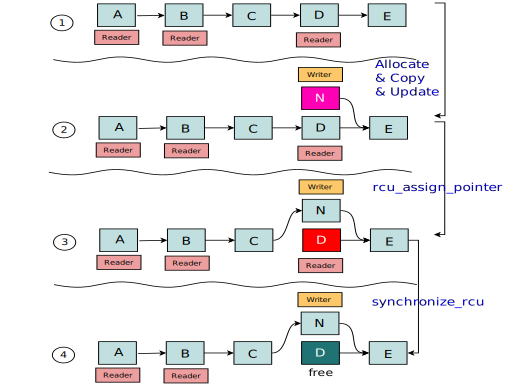
\includegraphics[width=1\textwidth]{fig/rcu/rcu_principle}
    \caption{RCU 예제}
  \label{fig:rcuprinciple}
\end{figure}


RCU의 기본 철학은 특정 시점에서 오브젝트를 복제해서 처리한다. 그림~\ref{fig:rcuprinciple}은 
이러한 RCU의 예를 보여준다.
그림에서 1단계에는 A, B, C, D, E 오브젝트 중 A, B, D 오브젝트를 리더들이 읽는 과정을 보여준다.
만약 이 순간 D 오브젝트를 수정하려 하면, RCU는 복사본을 할당 받고, 새로운 값인 오브젝트 N으로 수정을 한다.
그리고 다음 단계에서는 atomic한 연산을 통해서 오브젝트 C와 N을 연결한다. 
이 순간 오브젝트 D를 읽고 이는 리더와 다른 리더들은 아무런 블락 없이 계속 읽기를 수행할 수 있으며,
 동시에 업데이트까지 수행할 수 있어서 성능이 향상된다.
마지막으로 \code{synchroinze\_rcu()} 함수를 통해 리더가 읽기를 마칠 때 까지 기다리고, 읽기가 끝나면 
바로 \code{free()}를 수행한다. 
이 때 마지막 리더가 읽을 때 까지 기다리는 시간을 RCU에서는 grace period라 부른다. 


RCU는 기본적으로 3가지 특징을 가진다. 첫 번째로 Lock-free 리더이다.
실제로 RCU의 리더들은 아무런 락 또는 배리어(barrier)를 소유하지 않고 수행되며, 리드 구간에서는
 per-core 자료구조에 
단순히 enter/exit를 기록하여 수행한다. 
따라서, 락 발생하는 캐시 일관성 트래픽이 발생하지 않는다.
두번 째로, Single pointer update이다.
RCU의 writer는 atomic 명령으로 one pointer 업데이트를 수행한다.
이러한 특징으로 인해 여러 리더들과 한가지 업데이터가 동시에 동작할 수 있다.  
마지막으로, RCU는 delayed free를 수행한다.
노드를 바로 free를 하지 않고, 모든 리더들이 리드 구역을 벋어난 경우 까지 
기다린 후 해당 노드를 free한다.
이를 통해 안전하게 노드를 자원 해재할 수 있다. 

\begin{figure}[h]
    \centering
    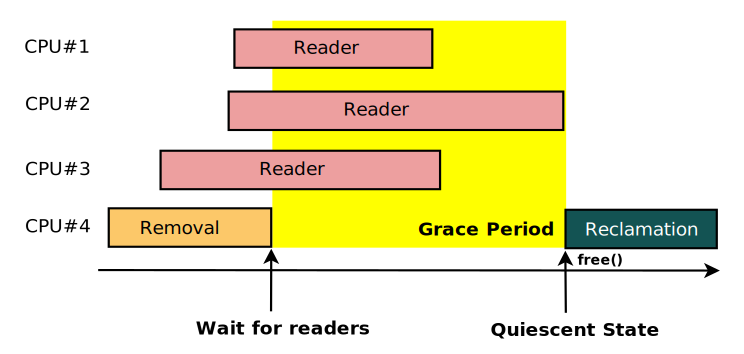
\includegraphics[width=1\textwidth]{fig/rcu/rcu_grace}
    \caption{RCU의 delayed free의 시점}
  \label{fig:rcu_grace}
\end{figure}

그림~\ref{fig:rcu_grace}는 RCU의 delayed free의 시점을 보여준다 . 



\begin{figure*}[h]
\begin{center}
\inputminted[linenos,fontsize=\footnotesize,
tabsize=4]{c}{src/rcu_list_data.c}
\end{center}
\caption{LDU의 동시적 삽제에 대한 알고리즘.}
\label{fig:gldulogicalupdate}
\end{figure*}



\begin{figure}[h!]
\begin{center}
\inputminted[linenos,fontsize=\footnotesize,
tabsize=4]{c}{src/rcu_list_search.c}
\end{center}
\caption{LDU의 동시적 삽제에 대한 알고리즘.}
\label{fig:gldulogicalupdate}
\end{figure}


\begin{figure}[h!]
\begin{center}
\inputminted[linenos,fontsize=\footnotesize,
tabsize=4]{c}{src/rcu_list_delete.c}
\end{center}
\caption{LDU의 동시적 삽제에 대한 알고리즘.}
\label{fig:gldulogicalupdate}
\end{figure}



\begin{figure}[h!]
    \centering
    \includegraphics[width=1\textwidth]{fig/rcu/rcu_list}
    \caption{공유 메모리 시스템}
  \label{shared_memory}
\end{figure}

\subsubsection{RLU}

RLU는 \ldots


\begin{figure}[h!]
    \centering
    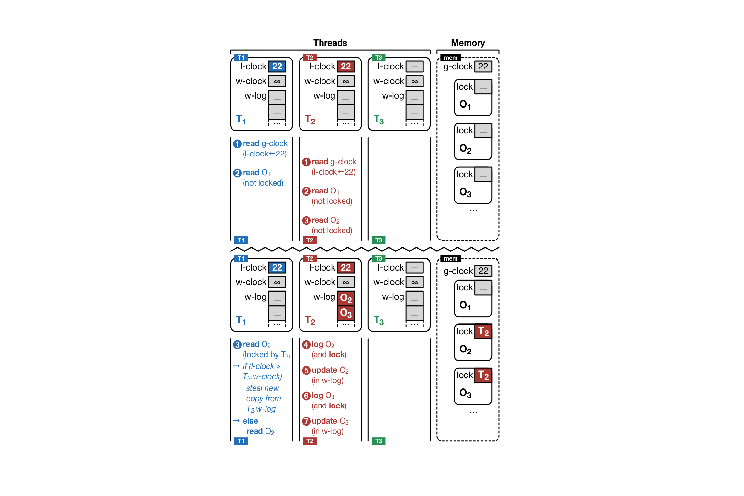
\includegraphics[width=1\textwidth]{fig/rlu/rlu_principle}
    \caption{공유 메모리 시스템}
  \label{shared_memory}
\end{figure}




\subsection{확장성 있는 자료구조}

Non-blocking 알고리즘은\ldots


\subsubsection{Harris Linked List}


Non-blocking 알고리즘은\ldots


\begin{figure}[h]
    \centering
    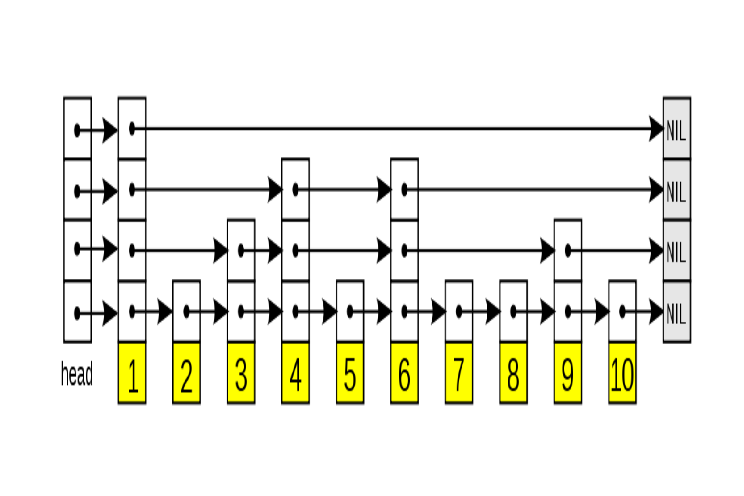
\includegraphics[width=1\textwidth]{fig/ds/skiplist}
    \caption{공유 메모리 시스템}
  \label{shared_memory}
\end{figure}




\subsubsection{Fraser Skip List}


\begin{figure}[h]
    \centering
    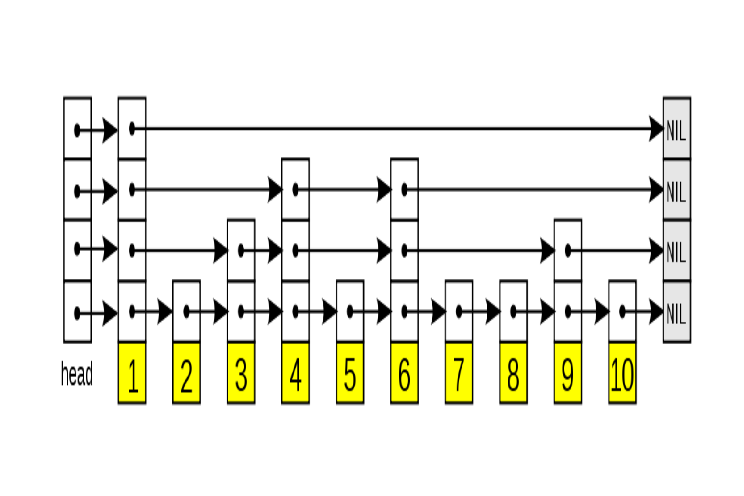
\includegraphics[width=1\textwidth]{fig/ds/skiplist}
    \caption{공유 메모리 시스템}
  \label{shared_memory}
\end{figure}



\subsubsection{Ctrus Tree}


\subsubsection{Time-stamp stack}
